\chapter{Anexo: Faster Whisper y Modelos de Transcripción}
\label{anexo-faster-whisper}

Este anexo explora Faster Whisper, una implementación optimizada del modelo Whisper de OpenAI para transcripción y traducción de voz a texto. Se analizan sus características principales, arquitectura, y se compara el rendimiento entre los diferentes modelos disponibles.

\section{Características Principales}
\label{sec:faster-whisper-features}

Faster Whisper representa una mejora significativa sobre la implementación original de Whisper, destacando por:

\begin{itemize}
	\item \textbf{Optimización CTranslate2}: Utiliza el toolkit CTranslate2 para optimizar la inferencia del modelo.
	\item \textbf{Menor Consumo de Memoria}: Reduce significativamente el uso de memoria mediante técnicas de cuantización.
	\item \textbf{Aceleración por Hardware}: Aprovecha eficientemente CPU y GPU mediante paralelización.
	\item \textbf{Detección de Voz}: Integra VAD (Voice Activity Detection) para mejorar la precisión.
\end{itemize}

\section{Arquitectura del Sistema}
\label{sec:faster-whisper-architecture}

\begin{figure}[H]
	\label{fig:whisper}
	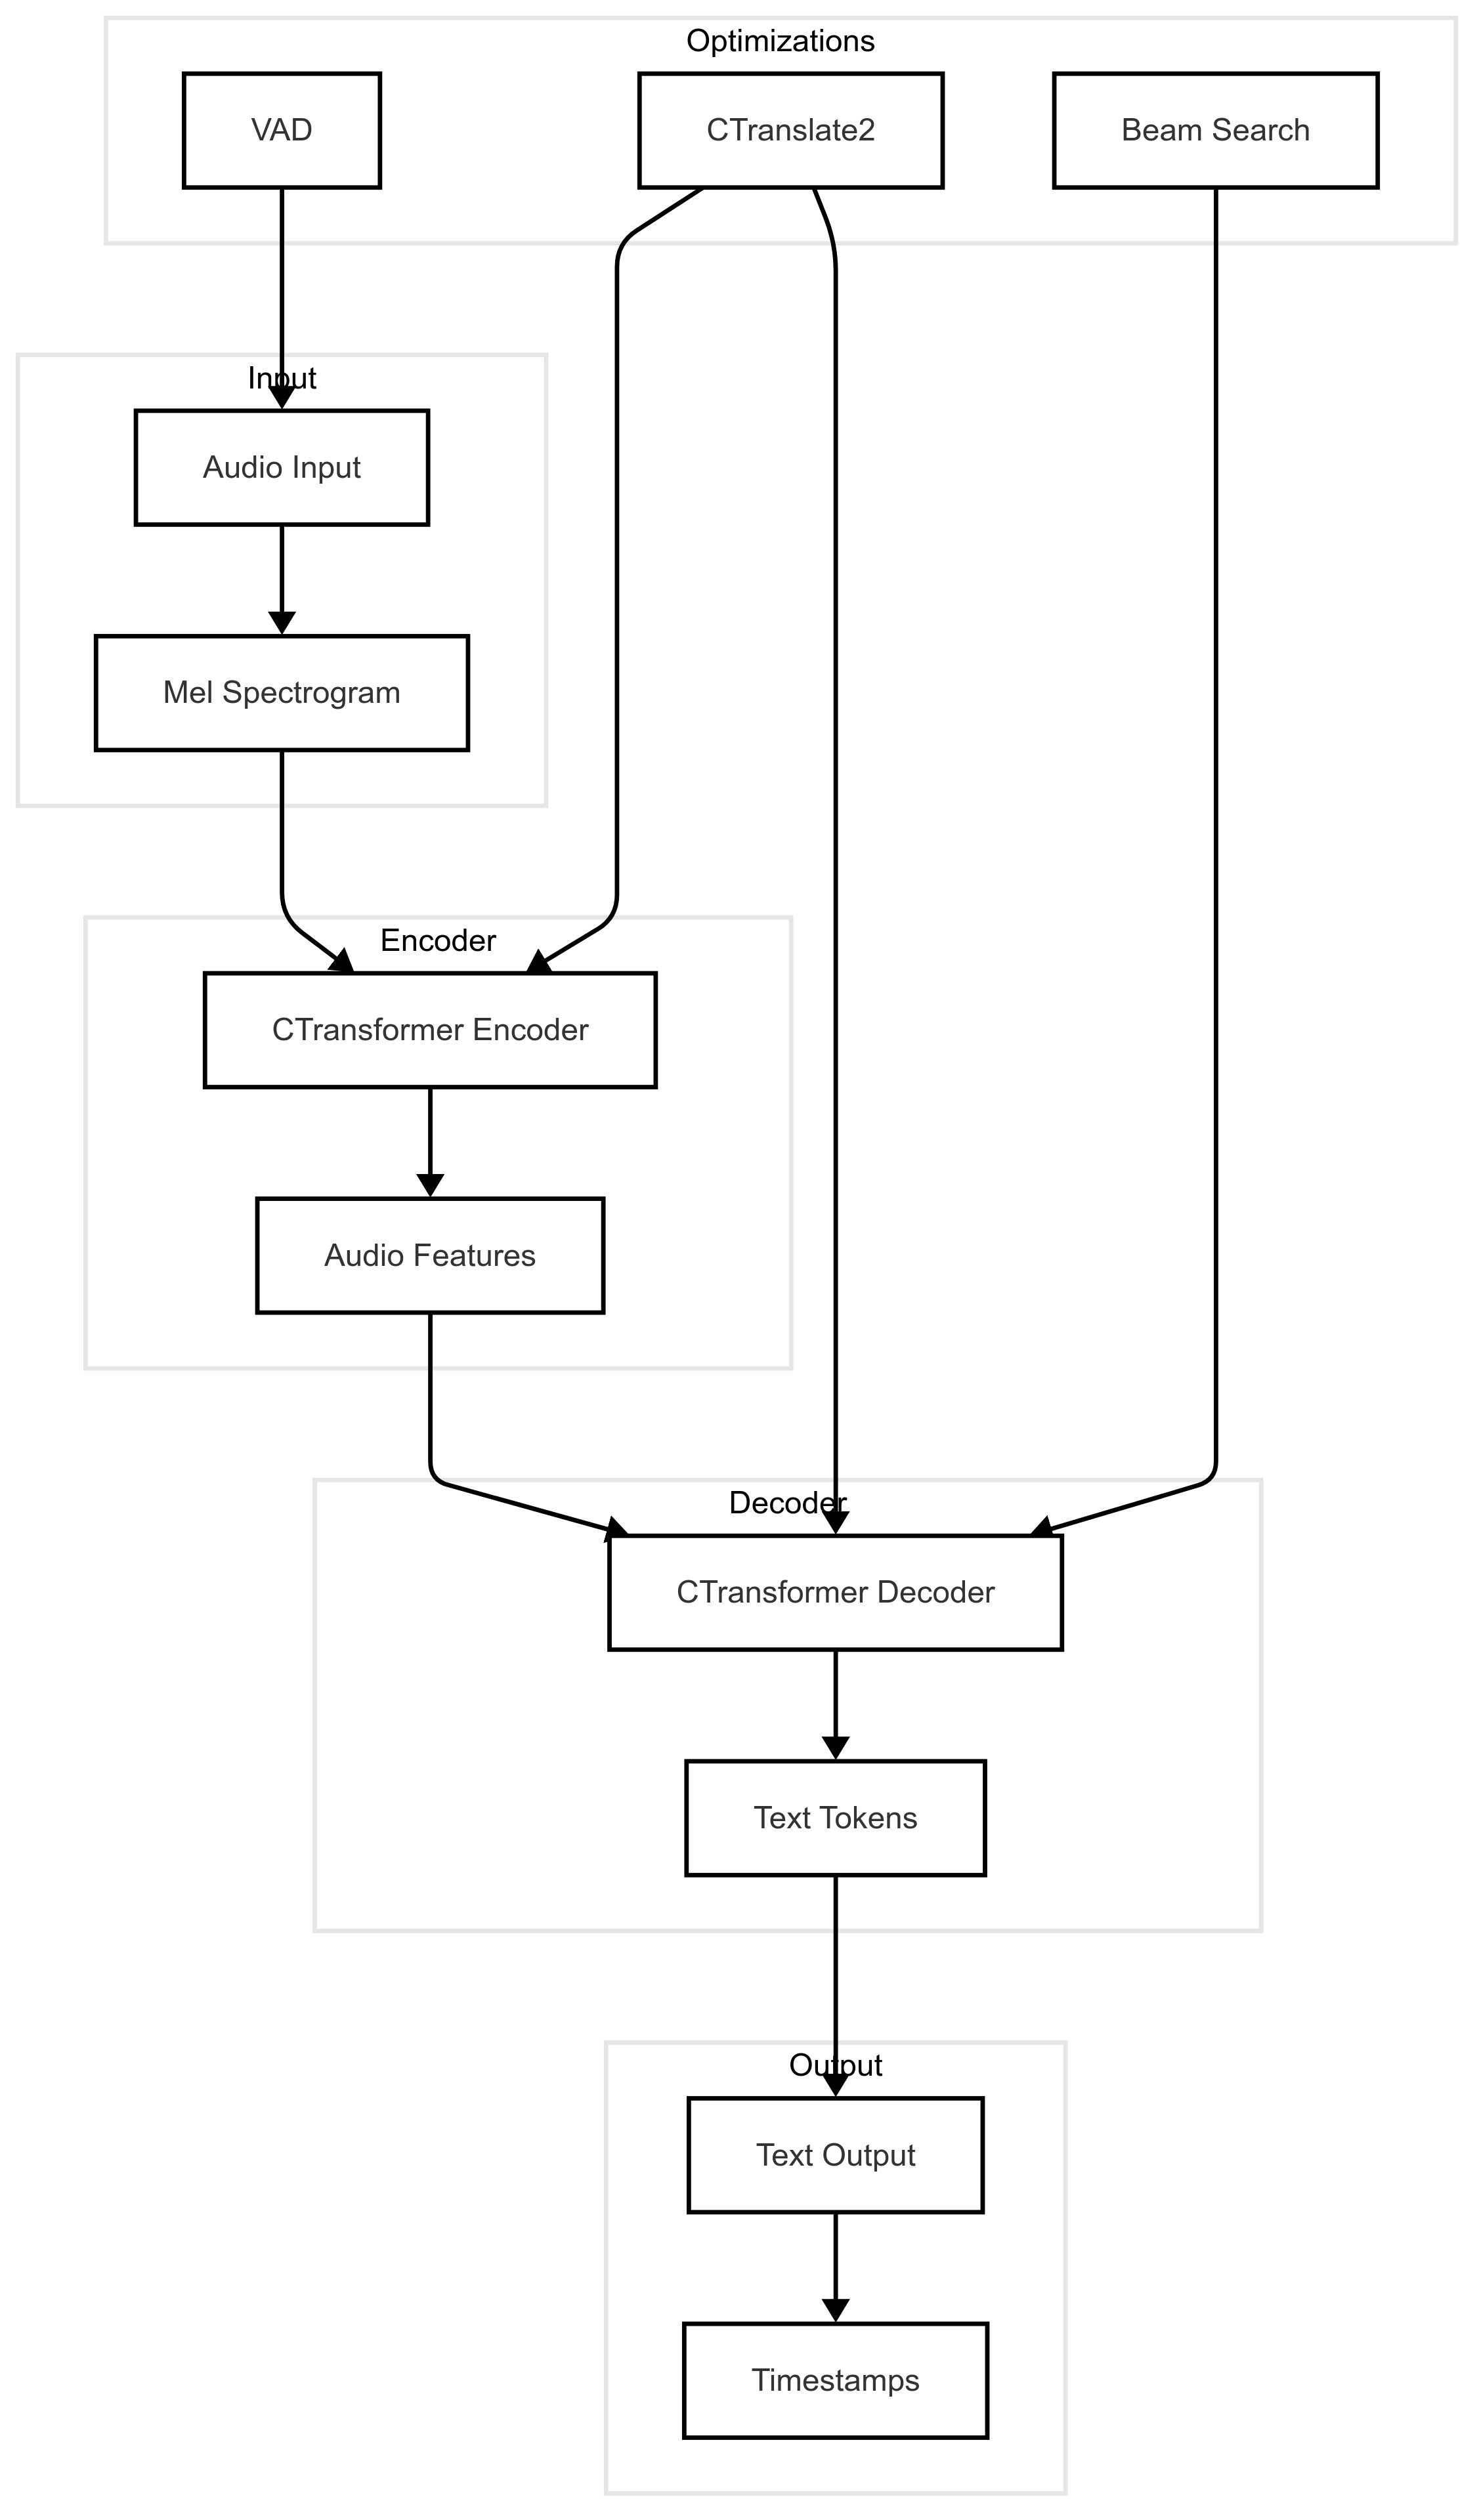
\includegraphics[width=0.8\textwidth]{figuras/whisper.png}
	\caption{Arquitectura de Faster Whisper}
\end{figure}

La arquitectura de Faster Whisper se compone de varios módulos especializados que trabajan en conjunto para proporcionar transcripción eficiente:

\subsection{Componentes Principales}
\label{subsec:main-components}

\subsubsection{Preprocesamiento de Audio}
El sistema procesa la entrada de audio mediante:
\begin{equation}
	\text{mel} = \text{log}(\max(\text{STFT}(x), \epsilon))
\end{equation}
donde STFT es la Transformada de Fourier de Tiempo Corto y $\epsilon$ es un valor pequeño para estabilidad numérica.

\subsubsection{CTransformer}
La implementación utiliza CTranslate2 para optimizar:
\begin{itemize}
	\item \textbf{Encoder}: Procesa el espectrograma mel en representaciones de audio.
	\item \textbf{Decoder}: Genera tokens de texto mediante atención cruzada.
\end{itemize}

\section{Comparativa de Modelos Whisper}
\label{sec:whisper-models-comparison}

\begin{table}[H]
	\label{tab:whisper-models}
	\begin{tabular}{|p{2cm}|p{2cm}|p{3cm}|p{3cm}|p{3cm}|}
		\hline
		\textbf{Modelo} & \textbf{Parámetros} & \textbf{RAM (FP16)} & \textbf{WER} & \textbf{Velocidad Relativa} \\
		\hline
		Tiny            & 39M                 & 1GB                 & 7.1\%        & 32x                         \\
		\hline
		Base            & 74M                 & 1.5GB               & 6.1\%        & 16x                         \\
		\hline
		Small           & 244M                & 2.5GB               & 5.2\%        & 8x                          \\
		\hline
		Medium          & 769M                & 4.5GB               & 4.3\%        & 4x                          \\
		\hline
		Large           & 1550M               & 7.5GB               & 3.6\%        & 1x                          \\
		\hline
	\end{tabular}
	\caption{Comparación de modelos Whisper}
\end{table}

\subsection{Características por Modelo}
\label{subsec:model-features}

\begin{itemize}
	\item \textbf{Tiny}:
	      \begin{itemize}
		      \item Ideal para dispositivos con recursos limitados
		      \item Mejor opción para transcripción en tiempo real
		      \item Rendimiento aceptable en condiciones de audio limpias
	      \end{itemize}

	\item \textbf{Base}:
	      \begin{itemize}
		      \item Balance entre rendimiento y recursos
		      \item Adecuado para aplicaciones web
		      \item Buen rendimiento en múltiples idiomas
	      \end{itemize}

	\item \textbf{Small}:
	      \begin{itemize}
		      \item Mejora significativa en precisión sobre Base
		      \item Soporte robusto para múltiples acentos
		      \item Detección confiable de cambios de idioma
	      \end{itemize}

	\item \textbf{Medium}:
	      \begin{itemize}
		      \item Alta precisión en condiciones desafiantes
		      \item Excelente rendimiento en audio con ruido
		      \item Capacidad avanzada de puntuación
	      \end{itemize}

	\item \textbf{Large}:
	      \begin{itemize}
		      \item Máxima precisión disponible
		      \item Mejor rendimiento en audios complejos
		      \item Capacidad superior de traducción
	      \end{itemize}
\end{itemize}

\section{Optimizaciones}
\label{sec:optimizations}

\subsection{Técnicas de Cuantización}
\label{subsec:quantization}

Faster Whisper implementa varias técnicas de cuantización:

\begin{itemize}
	\item \textbf{INT8}: Reduce el tamaño del modelo en 4x con mínima pérdida de precisión
	\item \textbf{INT16}: Balance entre precisión y tamaño
	\item \textbf{FLOAT16}: Máxima precisión con reducción de memoria
\end{itemize}

\subsection{Paralelización}
\label{subsec:parallelization}

El sistema implementa múltiples niveles de paralelización:

\begin{itemize}
	\item \textbf{Batch Processing}: Procesa múltiples segmentos simultáneamente
	\item \textbf{Thread Pooling}: Optimiza la utilización de CPU
	\item \textbf{GPU Acceleration}: Aprovecha CUDA para procesamiento paralelo
\end{itemize}

\section{Consideraciones de Implementación}
\label{sec:implementation-considerations}

\subsection{Selección de Modelo}
La elección del modelo debe considerar:

\begin{itemize}
	\item \textbf{Recursos Disponibles}: Memoria y capacidad de procesamiento
	\item \textbf{Requisitos de Latencia}: Tiempo de respuesta necesario
	\item \textbf{Precisión Requerida}: Tolerancia a errores
\end{itemize}

\subsection{Estrategias de Deployment}
Consideraciones para el despliegue:

\begin{itemize}
	\item \textbf{Edge Computing}: Procesamiento en dispositivo para menor latencia
	\item \textbf{Server-Side}: Mayor capacidad de procesamiento pero mayor latencia
	\item \textbf{Hybrid}: Combinación según necesidades específicas
\end{itemize}

\chapter{Anexo: Kokoro TTS}
\label{anexo-kokoro}

Este anexo explora Kokoro TTS, un modelo de síntesis de voz de código abierto que destaca por su eficiencia y calidad comparable a modelos más grandes, a pesar de contar con solo 82 millones de parámetros. El modelo implementa una arquitectura ligera basada en StyleTTS 2 e ISTFTNet, diseñada para ofrecer una síntesis de voz de alta calidad con recursos computacionales limitados.

\section{Arquitectura del Sistema}
\label{sec:kokoro-architecture}

La arquitectura de Kokoro TTS se fundamenta en dos componentes principales: StyleTTS 2 e ISTFTNet. Esta combinación permite una síntesis de voz eficiente mientras mantiene una alta calidad en la salida.

\subsection{Componentes Principales}
\label{subsec:kokoro-main-components}

\begin{itemize}
	\item \textbf{Misaki G2P}: Sistema de conversión de grafemas a fonemas que soporta múltiples idiomas.
	\item \textbf{Style Encoder}: Codifica las características de estilo de voz a partir de audio de referencia.
	\item \textbf{Decoder}: Genera características acústicas basadas en los fonemas y el estilo.
	\item \textbf{ISTFT Network}: Realiza la síntesis final del audio mediante transformada inversa de Fourier.
\end{itemize}

\section{Características Técnicas}
\label{sec:technical-features}

\subsection{Especificaciones del Modelo}
\begin{itemize}
	\item \textbf{Parámetros}: 82 millones
	\item \textbf{Arquitectura Base}: StyleTTS 2 + ISTFTNet
	\item \textbf{Licencia}: Apache 2.0
	\item \textbf{Formato de Audio}: 24kHz, mono
\end{itemize}

\subsection{Conjunto de Datos}
El entrenamiento se realizó exclusivamente con datos de audio permitidos:
\begin{itemize}
	\item Audio de dominio público
	\item Audio con licencias permisivas (Apache, MIT)
	\item Audio sintético de modelos comerciales
\end{itemize}

\section{Análisis de Voces}
\label{sec:voice-analysis}

\subsection{Sistema de Calificación}
\label{subsec:grading-system}

El sistema evalúa las voces mediante dos métricas principales:

\begin{itemize}
	\item \textbf{Calidad Objetivo}:
	      \begin{itemize}
		      \item A: Calidad excepcional
		      \item B: Buena calidad
		      \item C: Calidad aceptable
		      \item D: Calidad limitada
	      \end{itemize}

	\item \textbf{Duración del Entrenamiento}:
	      \begin{itemize}
		      \item HH: 10-100 horas
		      \item H: 1-10 horas
		      \item MM: 10-100 minutos
		      \item M: 1-10 minutos
	      \end{itemize}
\end{itemize}

\subsection{Distribución de Voces}
\label{subsec:voice-distribution}

\begin{table}[H]
	\centering
	\label{tab:voice-distribution}
	\begin{tabular}{|l|c|c|c|l|}
		\hline
		\textbf{Idioma}  & \textbf{F} & \textbf{M} & \textbf{Total} & \textbf{Calidad Media} \\
		\hline
		Inglés Americano & 11         & 9          & 20             & B-                     \\
		\hline
		Inglés Británico & 4          & 4          & 8              & C+                     \\
		\hline
		Japonés          & 4          & 1          & 5              & C+                     \\
		\hline
		Chino Mandarín   & 4          & 4          & 8              & D+                     \\
		\hline
		Español          & 1          & 2          & 3              & C                      \\
		\hline
		Francés          & 1          & 0          & 1              & B-                     \\
		\hline
		Hindi            & 2          & 2          & 4              & C                      \\
		\hline
		Italiano         & 1          & 1          & 2              & C                      \\
		\hline
		Portugués BR     & 1          & 2          & 3              & C                      \\
		\hline
	\end{tabular}
	\caption{Distribución y calidad de voces por idioma}
\end{table}

\section{Rendimiento y Limitaciones}
\label{sec:performance}

\subsection{Rangos Óptimos de Operación}
\label{subsec:optimal-ranges}

El rendimiento del modelo varía según la longitud del texto:
\begin{itemize}
	\item \textbf{Rango Óptimo}: 100-200 tokens
	\item \textbf{Rendimiento Reducido}: <20 tokens
	\item \textbf{Posible Aceleración}: >400 tokens
\end{itemize}

\subsection{Costos de Entrenamiento}
\label{subsec:training-costs}

El entrenamiento de Kokoro ha sido notablemente eficiente:
\begin{itemize}
	\item \textbf{Horas GPU}: 1000 horas en A100 80GB
	\item \textbf{Costo Total}: Aproximadamente \$1000 USD
	\item \textbf{Tasa Promedio}: \$1/hora
\end{itemize}

\section{Comparativa con Otros Modelos}
\label{sec:model-comparison}

\begin{table}[H]
	\centering
	\label{tab:model-comparison}
	\begin{tabular}{|l|c|c|c|c|}
		\hline
		\textbf{Modelo} & \textbf{Parámetros} & \textbf{Voces} & \textbf{Idiomas} & \textbf{Licencia} \\
		\hline
		Kokoro          & 82M                 & 54             & 8                & Apache            \\
		\hline
		Coqui           & 1000M               & 1087           & 100+             & MIT               \\
		\hline
		Bark            & 900M                & 100+           & 100+             & MIT               \\
		\hline
	\end{tabular}
	\caption{Comparación con modelos TTS similares}
\end{table}